\documentclass[11pt,a4paper]{article} 

\usepackage[T1]{fontenc}
\usepackage[utf8]{inputenc}
\usepackage{lmodern}
\usepackage[french,english]{babel}

\usepackage{amsthm}
\usepackage{float}
\usepackage{lmodern}%pour un meilleur rendu des polices
\usepackage{verbatim}%du texte non interprt
\usepackage[cmex10]{amsmath}
\usepackage{amssymb}%maths
\usepackage{xspace}
\usepackage[dvipsnames,svgnames,table]{xcolor}
\usepackage{listings}
\usepackage{fancyhdr}
\usepackage{etoolbox}
\usepackage{titlesec}
\usepackage{titletoc}
\usepackage{lastpage}
\usepackage[bookmarks=true,bookmarksnumbered=true]{hyperref}
\usepackage{ctable} % for \specialrule command
\usepackage{cite}
\usepackage{algorithm2e}
\usepackage{alltt}
\usepackage{array}
\usepackage{mdwmath}
\usepackage{mdwtab}
\usepackage{eqparbox}
\usepackage[caption=false,font=normalsize,labelfont=sf,textfont=sf]{subfig}
\usepackage{dblfloatfix}
\usepackage{url}
\usepackage{tipa}
\usepackage{stmaryrd}
\usepackage{upgreek}
\usepackage{mathrsfs}

%\usepackage{natbib}
%\usepackage[pdftex]{graphicx}
%\usepackage{framed}
%\usepackage[usenames]{color}

\graphicspath{{img/}}
\DeclareGraphicsExtensions{.pdf,.jpeg,.jpg,.png}

%% taille du papier
\textwidth 16 true cm
\textheight 24 true cm
\addtolength{\hoffset}{-1.5cm}
\addtolength{\voffset}{-1.5cm}

%-------- couleurs
\definecolor{grisf}{rgb}{.47,.47,.47} % barre de droite gris fonce
\newcommand{\colorc}{\color{MidnightBlue}}
\newcommand{\colorb}{\color{NavyBlue}}
\newcommand{\colora}{\color{Cerulean}}

%----------- sections et TOC
% chapitres
\titleformat{\chapter}[display]
  {\normalfont\sffamily\bfseries\huge\colora\centering}{\thechapter}{1ex}
  {{\titlerule[1pt]}\vspace{1.3ex}}[\vspace{1ex}{{\titlerule[1pt]}}]
  
% chapitres etoiles  
\titleformat{name=\chapter,numberless}[display]
  {\normalfont\sffamily\bfseries\LARGE\colora\centering}{}{1ex}
  {{\titlerule[1pt]}\vspace{1.3ex}}[\vspace{1ex}{\titlerule[1pt]}\vspace{2ex}]
  
% sections  
\titleformat{\section}[hang]{\Large\normalfont\sffamily\bfseries\colora}{{\thesection\, }}{0 em}
  {}[{\titlerule[1pt]}\vspace{1ex}]

  
% sous section, sous sous sec, paragraphes  
\titleformat{\subsection}[hang]{\Large\normalfont\sffamily\bfseries\colorc}{{\thesubsection\, }}{0 em}
  {}[{\titlerule}\vspace{.7ex}]
\titleformat{\subsubsection}[hang]{\normalfont\sffamily\bfseries\large}{{\thesubsubsection\, }}{0 em}
  {}[{\color{grisf}\titlerule}\vspace{3pt}]
\titleformat{\paragraph}[runin]{\normalfont\sffamily\bfseries\colorb}{}{0 em}
  {\indent}



%----------------- fancy headers -------------%

\makeatletter
\patchcmd{\@fancyhead}{\rlap}{\color{grisf}\rlap}{}{}
\patchcmd{\headrule}{\hrule}{\color{grisf}\hrule}{}{}
\patchcmd{\@fancyfoot}{\rlap}{\color{grisf}\rlap}{}{}
\patchcmd{\footrule}{\hrule}{\color{grisf}\hrule}{}{}
\makeatother

                                                                    
\fancyhf{}
\fancyhead[R]{\sffamily Article summary }
\fancyfoot[R]{\sffamily\small{\thepage/\pageref{LastPage}}}
\fancyhead[L]{\sffamily\small{Jean-Baptiste Keck}}
\fancyfoot[L]{\sffamily\small{M2 MSIAM -- High Performance Exact Computing -- 2014-2015}}
\renewcommand{\headrulewidth}{0.2pt} %0.4
\renewcommand{\footrulewidth}{0.2pt} %0
\addtolength{\headheight}{0.pt}

\fancypagestyle{plain}{
  \fancyhead{}
  \renewcommand{\headrulewidth}{0pt}
  }
     
  %-- macros --%   
  \def\hlinewd#1{%
      \noalign{\ifnum0=`}\fi\hrule \@height #1 %
  \futurelet\reserved@a\@xhline} 

  
  
  %------------------- front page ------------------%
  \title{
      \bsc{Paper Review}
      \vskip 1cm
      {\colorb\textbf{How to Compute Fast a Function and All Its Derivatives}}
      \vskip 1cm
      {\colorc\textit{A variation on the theorem of Bauer-Strassen}}
  }
\author{%
    Jean-Baptiste \bsc{Keck}
    \vskip 0.5cm
    \bsc{M2 Msiam}
}
%\date{27 janvier 2014}
\makeatletter

\def\maketitle{%
    %\thispagestyle{empty}%
    \begin{flushleft}
        \normalfont\LARGE\par
    \end{flushleft}
    \vskip 3cm
    \begin{center}%
        {\colora\specialrule{.2em}{0em}{0em}}
        \vskip 1cm
        {\Huge \@title}%
        \vskip 1cm
        {\colora\specialrule{.2em}{0em}{0em}}
        \vskip 5cm
        {\Huge \@author\par}%
        \vskip 2cm
        {\Huge \@date\par}%
        \vskip 1cm

    \end{center}%
    \clearpage
}

\renewcommand{\ccite}[1]{\textbf{\cite{#1}}}
\renewcommand{\pd}[2]{\dfrac{\partial #1}{\partial #2}}
\renewcommand{\od}[2]{\dfrac{\mathscr{D}_a #1}{\mathscr{D} #2}}
\renewcommand{\tensor}[1]{\mathbf{#1}}
\renewcommand{\vector}[1]{\overrightarrow{#1}}

\renewcommand{\Tau}{\tensor{\mathlarger{\uptau}}}
\renewcommand{\v}{\vector{u}}
\renewcommand{\W}{\tensor{W\left( \v \right)}}
\renewcommand{\D}{\tensor{D\left( \v \right)}}
\renewcommand{\grad}{\vector{\nabla}}
\renewcommand{\gradv}{\tensor{\nabla\v}}
\renewcommand{\div}[1]{div \left( #1 \right)}}
\renewcommand{\divv}[1]{\vector{div} \left( #1 \right)}
\renewcommand{\UU}{\mathcal{U}}
\renewcommand{\M}{\mathcal{M}}
\renewcommand{\A}[2]{\mathcal{A}_{#1}\left( #2 \right)}
\renewcommand{\Uu}{\UU^{n}}
\renewcommand{\Uv}{\UU^{n+\theta}}
\renewcommand{\Uw}{\UU^{n+1-\theta}}
%%%%%%%

\begin{document}
\pagestyle{fancy}

%\maketitle

%\tableofcontents
%\clearpage

\section{Operator notations} 

$$
\begin{array}{l l l c c l c l c}
    \gradv&
    =&
    \underbrace{\D}_{deformation\ rate}&
    +&
    \underbrace{\W}_{vorticity}&
    =&
    \left[\dfrac{\gradv + \gradv^T}{2}\right]&
    +&
    \left[\dfrac{\gradv - \gradv^T}{2}\right]
    \\
    \\
    \Tau_&
    =&
    \underbrace{\Tau_d}_{\underset{(shear)}{deviatoric\ stress}}&
    +&
    \underbrace{\Tau_s}_{\underset{(pressure)}{hydrostatic\ stress}}&
    =&
    \left[\Tau - \dfrac{1}{d}tr(\Tau)\tensor{I_d}\right]&
    +&
    \left[\dfrac{1}{d}tr(\Tau)\tensor{I_d}\right]
\end{array}
$$

$
\forall a \in \left[ -1,1\right] \hspace{0.5cm}
\tensor{\od{\Tau}{t}} = \pd{\Tau}{t} + \left(\v . \grad \right) \Tau + \tensor{\beta_a \left( \Tau, \gradv \right)}
\textrm{ is the Jaumann objective stress rate.}
$
\vskip 0.5cm
$
\hskip 2.6cm
\beta_a \left( \Tau, \gradv \right) = \Tau . \W - \W . \Tau - a \left[ \D.\Tau + \Tau . \D \right]
$
\vskip 0.5cm
$
\forall \; \Tau \in \mathbb{R}^{d \times d} \hskip 0.5cm
|\Tau|^2=
\Tau : \Tau =
tr\left(\Tau^T \Tau \right) =
\displaystyle \sum_{1\leq i,j \leq d}\Tau_{ij}^2 \hskip 0.5cm \textrm{(usual matrix Euclidean norm)}
$
           
\clearpage
\section{Model parameters and notations}

{\colorb\textbf{Model parameters:}}
\vskip 0.5cm
\indent\textbf{Dimension: } $d \in \left\{ 2,3\right\}$
\vskip 0.2cm
\indent\textbf{Jaumann operator parameter: } $a \in \left[-1,1\right]$
\vskip 0.2cm
\indent\textbf{Fluid properties:}
\vskip 0.3cm
\left[
\begin{array}{l l}
    $\rho$ &solution\ density&
    $\eta_s$ &solvent\ \ viscosity&
    $\eta_m$ &polymer\ viscosity&
    $\lambda$ &elastic\ relaxation\ time&
    $\Tau_Y$ &yield\ stress&
\end{array}
\right]
\Leftrightarrow
\left[
\begin{array}{l l l l}
    
    $L,V$&=&\multicolumn{2}{l}{Caracteristic\ length\ and\ velocity}&
    $W_e&=& \lambda V/L$ &Weissenberg\ number&
    $B_i&=& \Tau_YL/\eta_m$ &Bingham\ number&
    $R_e&=& \rho VL/(\eta_m+\eta_s) $ &Reynolds\ number&
    $\alpha&=&\eta_m/(\eta_m+\eta_s)$ &Retardation\ parameter&
\end{array}
\right]

\vskip 0.5cm

\noindent{\colorb\textbf{Notations:}}\\

\textbf{Cauchy stress tensor:} $\Tau_{tot} = \underbrace{\Tau}_{elastic\ stress} - \underbrace{p\tensor{Id}}_{pressure} + \underbrace{2\eta_s\D}_{viscous\ friction}$

\vskip 0.5cm
\indent\textbf{Yield response:} $\mathcal{K}(|\Tau_d|) = \left[ \dfrac{|\Tau_d| - Bi}{n |\Tau_d|}\right]_+^n = \textrm{\textbf{max}}\left(0, \; 1 - \dfrac{B_i}{|\Tau_d|} \right) \textrm{ with } n = 1 \textrm{ (Bingham viscoplasticity)}.$\\
\vskip 0.1cm
\indent\hskip 3.1cm $\Tau_d$ is the elastic shear stress

\vskip 0.5cm

\clearpage
\section{Domain:} 

\begin{table}[h]
    \centering
    \begin{array}{l c c c c c r}
        $\mathlarger{\Omega \subset \mathbb{R}^d}$ &
        &&   
        $\mathlarger{\partial\Omega = \Gamma_d \cup \Gamma_n \cup \Gamma_s}$ &
        &&
        $\underbrace{\mathlarger{\partial\Omega_- = \Gamma_- = \left\{x\in \partial\Omega\ |\ \v.\vector{n} < 0\right\}}}_{upstream\ boundary} $
    \end{array}
\end{table}

\begin{figure}[h!]
   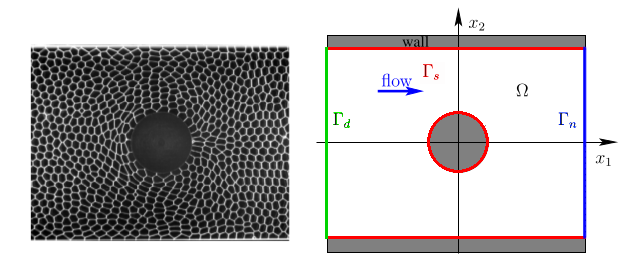
\includegraphics[scale=0.7]{domain.png}
   \caption{Experimental configuration}
\end{figure}


\clearpage
\section{Model equations}
Find $\ \mathcal{U} = (\Tau,\v, p) : \; \left]0,T\right[ \times \Omega \rightarrow \mathbb{R}^{d\times d} \times \mathbb{R}^d \times \mathbb{R}$ such that :

$$
(P) \Leftrightarrow 
\[
   \left \{
       \begin{array}{l l l l}
       (1)&
           W_e\left[\textcolor{blue}{\tensor{\od{\Tau}{t}}}\right] + \textcolor{red}{\mathcal{K} \left( | \Tau_d | \right) \Tau} - 2\alpha \tensor{D(\v)}&
       =& 0_{\mathbb{R}^{d \times d}}}&
           &&&&       
       (2)&
           Re\left[ \pd{\v}{t} + \textcolor{RoyalPurple}{\left(\v . \grad \right) \v} \right] \underbrace{-\divv{\Tau -p\tensor{I}_d+2\eta_s\tensor{D(\v)}}}_{ -\divv{\Tau_{tot}} = -\divv{\Tau} + \grad p - (1-\alpha)\Delta\v}&
           =&
       0_{\mathbb{R}^d}&
         &&&&       
           (3)& \div{\v} &=& 0_\mathbb{R}&
         &&&&
       (4)& \v = \vector{v_{\Gamma_d}} \hskip 0.75cm \textrm{ in } \left] 0,T \right[ \times \Gamma_d
   \hskip 2.6cm \v . \vector{n} = 0\textrm{ in } \left]0,T[ \times \Gamma_s&&&
         &&&&
   (5)& \vector{F} = \Tau \vector{n} = 0 \textrm{ in } \left]0,T\right[ \times \Gamma_n
       \hskip 0.5cm 
   \vector{F_t} = \Tau \vector{n} - \Tau_{nn} \vector{n}} = 0 \textrm{ in } \left]0,T[ \times \Gamma_s&&&
        &&&&
   (6)& \Tau = \Tau_- \hskip 1.05cm \textrm{ in } \left]0,T\right[ \times \Gamma_-
   \end{array}
   \right .
\]
$$

\begin{figure}[h!]
   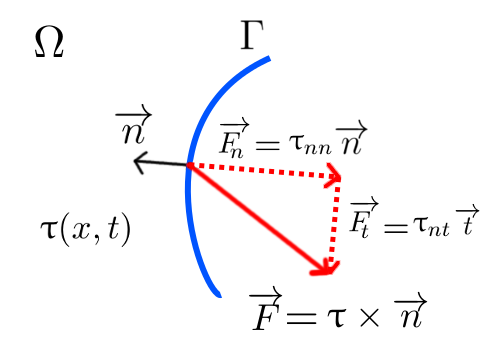
\includegraphics[scale=0.5]{force.png}
\end{figure}

\clearpage

\section{Algorithm}

{\colorb \textbf{Operator splitting:}}

\vskip 0.5cm

$(P) \Leftrightarrow$ Find $\ \mathcal{U} = (\Tau,\v, p) : \; \left]0,T\right[ \times \Omega \rightarrow \mathbb{R}^{d\times d} \times \mathbb{R}^d \times \mathbb{R}$ such that :

\vskip 0.2cm
\hskip 1.3cm
    $\[
        \left\{
            \begin{array}{l}
                \M \pd{\UU}{t} + \A{}{\UU}= 0_{\mathbb{R}^{d\times d}\times \mathbb{R}^d \times \mathbb{R}} &
                &
                (4) \hskip 0.5cm (5) \hskip 0.5cm (6) \hskip 0.5cm \textrm{(Boundary conditions)}
            \end{array}
            \right.
        \]$

        \vskip 0.5cm
\hskip 1.0cm with $\M = \[
    \left [
       \begin{array}{c c c}
           W_e&0&0&
           0&R_e&0&
           0&0&0&
       \end{array}
    \right ]
    \textrm{ and } \A{}{\UU} = \A{1}{\UU} + \A{2}{\UU}
\]$

\vskip 0.5cm
$$
\A{}{\UU} = 
\underbrace{
    \left[\begin{array}{c}
            \textcolor{red}{\mathcal{K} \left( | \Tau_d | \right) \Tau} - 2\alpha \tensor{D(\v)}&
            -\divv{\Tau} + \grad p - (1-\alpha)\Delta\v&
            \div{\v}&
\end{array}\right]}_{\A{1}{\UU}\ contains\ all\ viscoplastic\ effects}
+
\underbrace{
    \left[\begin{array}{c}
           W_e\left[\textcolor{blue}{\left(\v . \grad \right) \Tau + \tensor{\beta_a \left( \Tau, \gradv \right)}}\right]&
           0&
           0&
\end{array}\right]}_{\A{2}{\UU}\ contains\ all\ viscoelastic\ effects}
$$

\clearpage
\section{Algorithm}

{\colorb $\mathbf{\Theta}$ \textbf{- Scheme :}}


\end{document}




 
 
     
     
 
 
 
 
 
 
 
 
 
